\chapter{GPS Variation Estimation}
\label{cha:GPS-variation-estimation}

The main component of the dataset is the GPS positional update events from the vehicles.
They contribute to 95\% of the events in the data, as shown by Figure \ref{fig:types-barplot} in Section \ref{sec:data-structure}.
An interesting high-level problem is thus the estimation of the variance in the GPS positions.
The hypotheses are that the GPS positions vary depending on:
\begin{enumerate}
    \item \textit{Environment (Spatial Locality):} 
    The surrounding environment impacts the visibility of GPS satellites. \todo{source?}
    For example, in an environment with a lot of reflections and obstacles, the precision of the GPS position will decrease.
    On the other hand, in open fields the precision will increase, as there are fewer obstacles blocking the GPS satellite signals.
    The environment can vary between different road segments, but also inside one road segment, e.g., a road can be partly covered by houses or trees.
    The variance could either be seen as continuous, where each point on the journey has its own variance, or as road segments, where each road segment has its own variance.
    In the continuous case, neighbouring pairs of points would be connected and thus exhibit more similar variance, depending on the distance between the points (granularity) in a journey.
    In the case of road segments, different segments would exhibit a, potentially, larger difference in variance.
    
    Road segments could either be created geographically, e.g., a segment is the road between two bus stops or between crossings, or contextually from the output of the continuous case.
    A geographical road segmentation would most likely get a higher average variance, as the environment could change within the segment.
    The contextual segmentation would look at sequences of points in the journey, and group the sequential points which exhibit similar variance.
    The result would potentially be segments where the inherent variance of each segment is lower than between different segments.

    Figure \ref{fig:gps-variation} illustrates how the GPS variance can differ for different road segments.
    In the shown scenario, the difference between geographical segmentation between crossings and contextual segmentation would be minor, as the variance seems to be similar for a given road segment.
    However, the difference would be major if the geographical segmentation was done between bus stops.
    The number of road segments would be higher in the crossing-geographical approach than in the contextual approach, as, for example, "Järnvägsgatan" has many crossings but exhibit similar variance. 
    

    \item \textit{GPS Sensor Calibration:}
    Each bus has its own GPS sensor, where different buses could have different models with their own calibrations.
    In the general case the different GPS sensors show small variance due to different calibrations.
    However, occasionally they can vary, e.g., by some constant factor, as shown in Figure \ref{fig:gps-sensor-calibration}.
    The single orange-coloured bus journey seems to have a constant offset compared to the rest of the journeys for that particular bus line.
    The shown scenario is quite extreme, as the offset is large enough to cause problems with the Bus Stop Detection Algorithm in the "Internal Analysis" component.
    No bus stops are detected in this particular scenario.
    These extreme situations can thus be detected by combining the positional events with the bus stop events.
    However, differences in calibrations which yield smaller offsets cannot be detected with this combining approach.


    \item \textit{Time:}
    The timestamp of the position events affects the precision of the GPS sensor.
    At a single given point of the journey the precision could vary depending on the positions of satellites and the amount of satellites visible.
    The hypothesis is that there is a constant bias to the GPS positions depending on the timestamp.
    The positions of the satellites thus cause a small offset to occur in the GPS position.
    This parameter probably has some periodicity, which could be fitted using a Gaussian Process with a periodical kernel.
    
\end{enumerate} 


\begin{figure}[ht!]
    \centering
    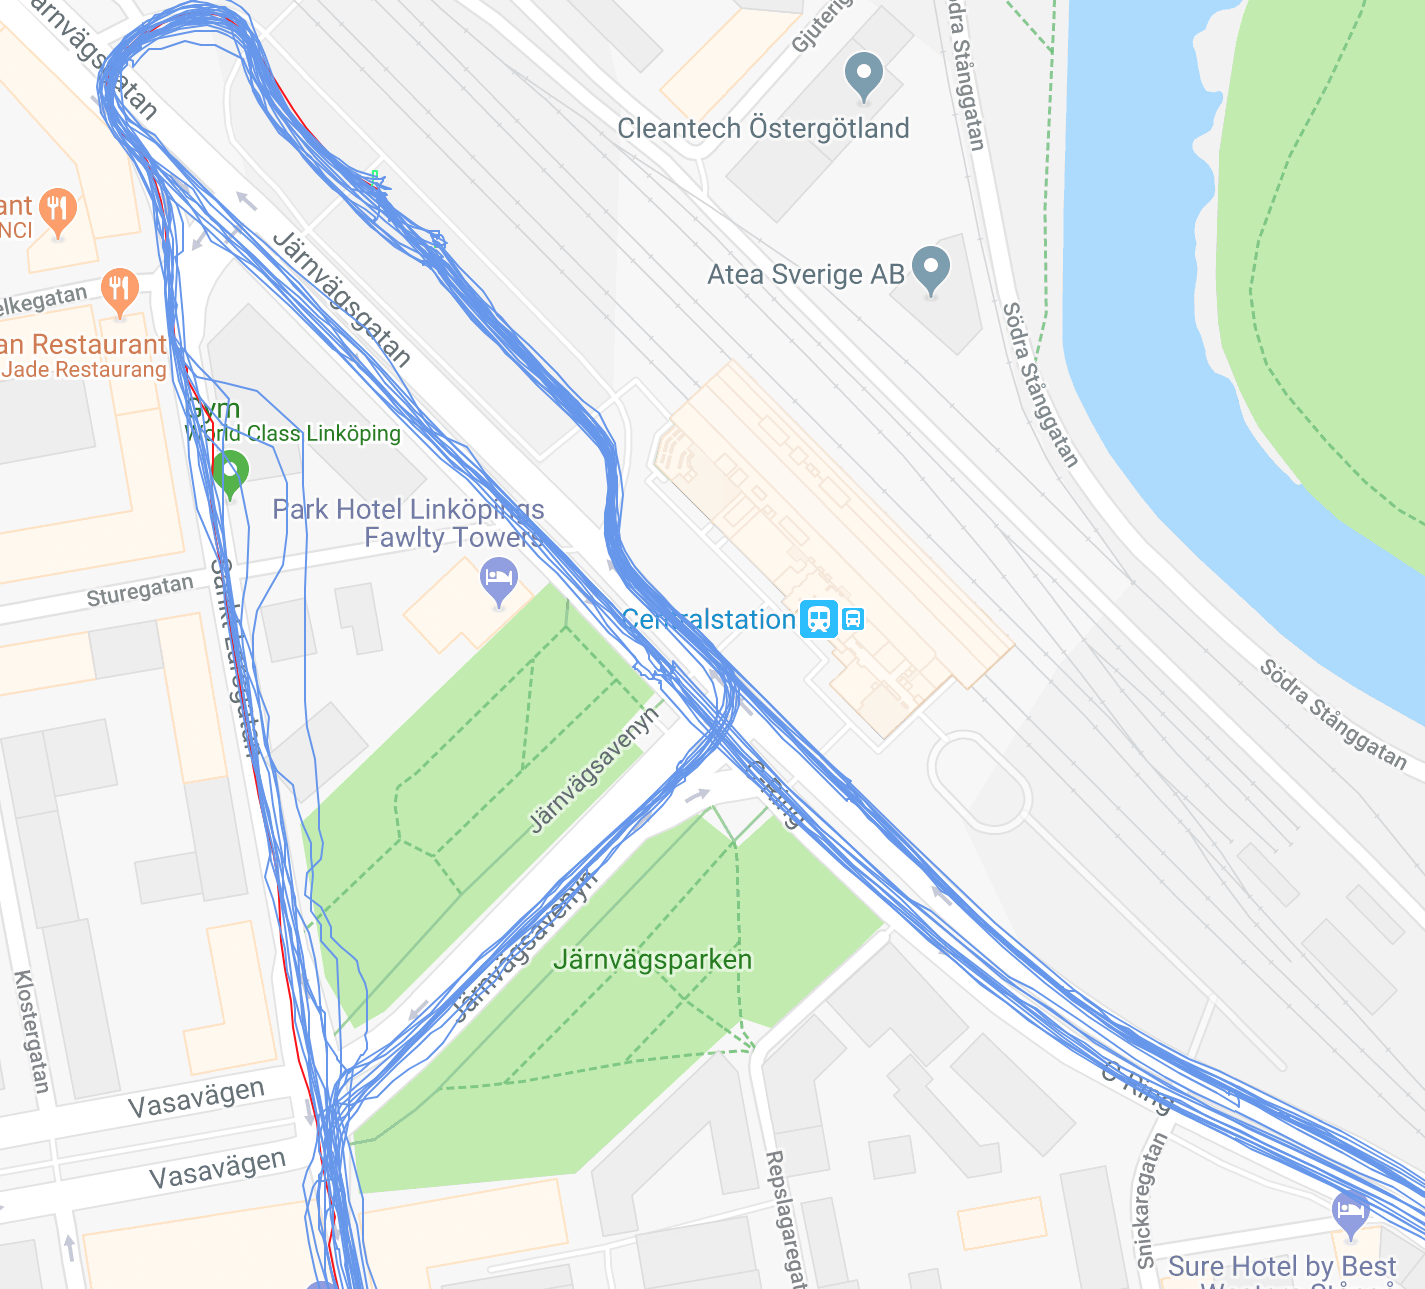
\includegraphics[width=0.9\textwidth]{figures/gps_variation}
    \caption[Visualisation of multiple journeys by different buses in the same area]
    {\small Visualisation of multiple journeys by different buses in the same area.
    Each blue line is a journey in the "Started" state.
    The variance differs between different road segments, as shown around "World Class Linköping" compared to "Järnvägsgatan".}
    \label{fig:gps-variation}
\end{figure}

\begin{figure}[ht!]
    \centering
    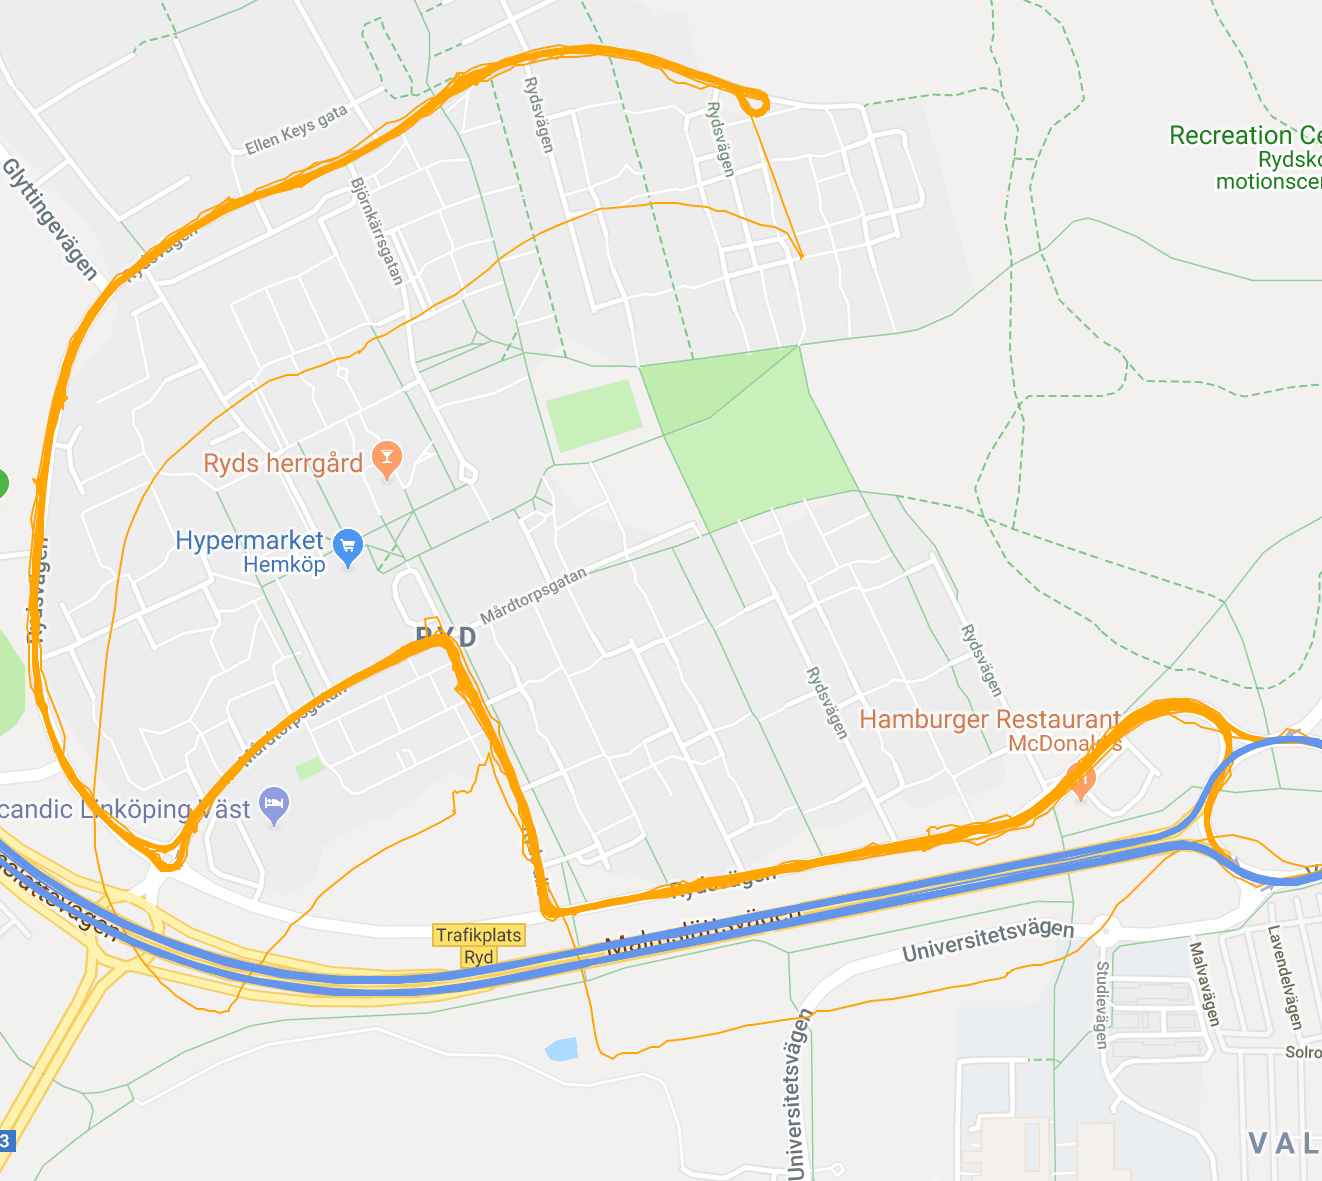
\includegraphics[width=0.9\textwidth]{figures/gps_sensor_calibration}
    \caption[Illustrates the case of a poorly calibrated GPS sensor on an individual bus]
    {\small Illustrates the case of a poorly calibrated GPS sensor on an individual bus.
    The orange lines creating the thicker line are all the other journeys for the same bus line, but done by other buses.
    The thin orange line is one bus with an extremely poorly calibrated GPS sensor.
    It seems to have a constant offset compared to the rest.
    This real-world scenario shows that the calibration of GPS sensors is important in order to produce useful data.}
    \label{fig:gps-sensor-calibration}
\end{figure}

\subsection{Road Segment Data}
Google Maps provides a Roads API\footnote{https://developers.google.com/maps/documentation/roads/intro} to map GPS coordinates to the closest road segment.
The road segments could, for example, be used to create a model calculating the orthogonal variance of GPS coordinates with respect to the road segments.
\todo{Bild?}
However, the variance of GPS positions does not only occur orthogonal to a given road segment. \todo{Vart vill jag komma med det här?} 

Manual inspection of journeys done in the pre-processing step highlights scenarios with discrepancies between roads in Google Maps and actual roads the buses drove.
The Google Maps roads are in these scenarios usually incorrectly drawn or has missing roads.
Figure \ref{fig:gps-map-problem} shows such a real-world example.
The discrepancies would cause problems if used naïvely together with the Google Maps Roads API.
These journeys would have to be detected and either handled or ignored.
The detection could be done by looking at the distances to the closest Google Maps Roads segments.
The distances would be roughly similar for all the journeys, as in Figure \ref{fig:gps-map-problem}.
Since the distances would be roughly similar they could be averaged and interpreted as a bias to the roads.
Applying the bias-interpretation methodology would result in a more generalised model using the Google Maps Roads API.
Ignoring the journeys with discrepancies could also be seen as feasible, given that the occurrence is rare.
Before using the simpler approach of ignoring journeys with discrepancies, a deeper analysis needs to be conducted.

\begin{figure}[ht!]
    \centering
    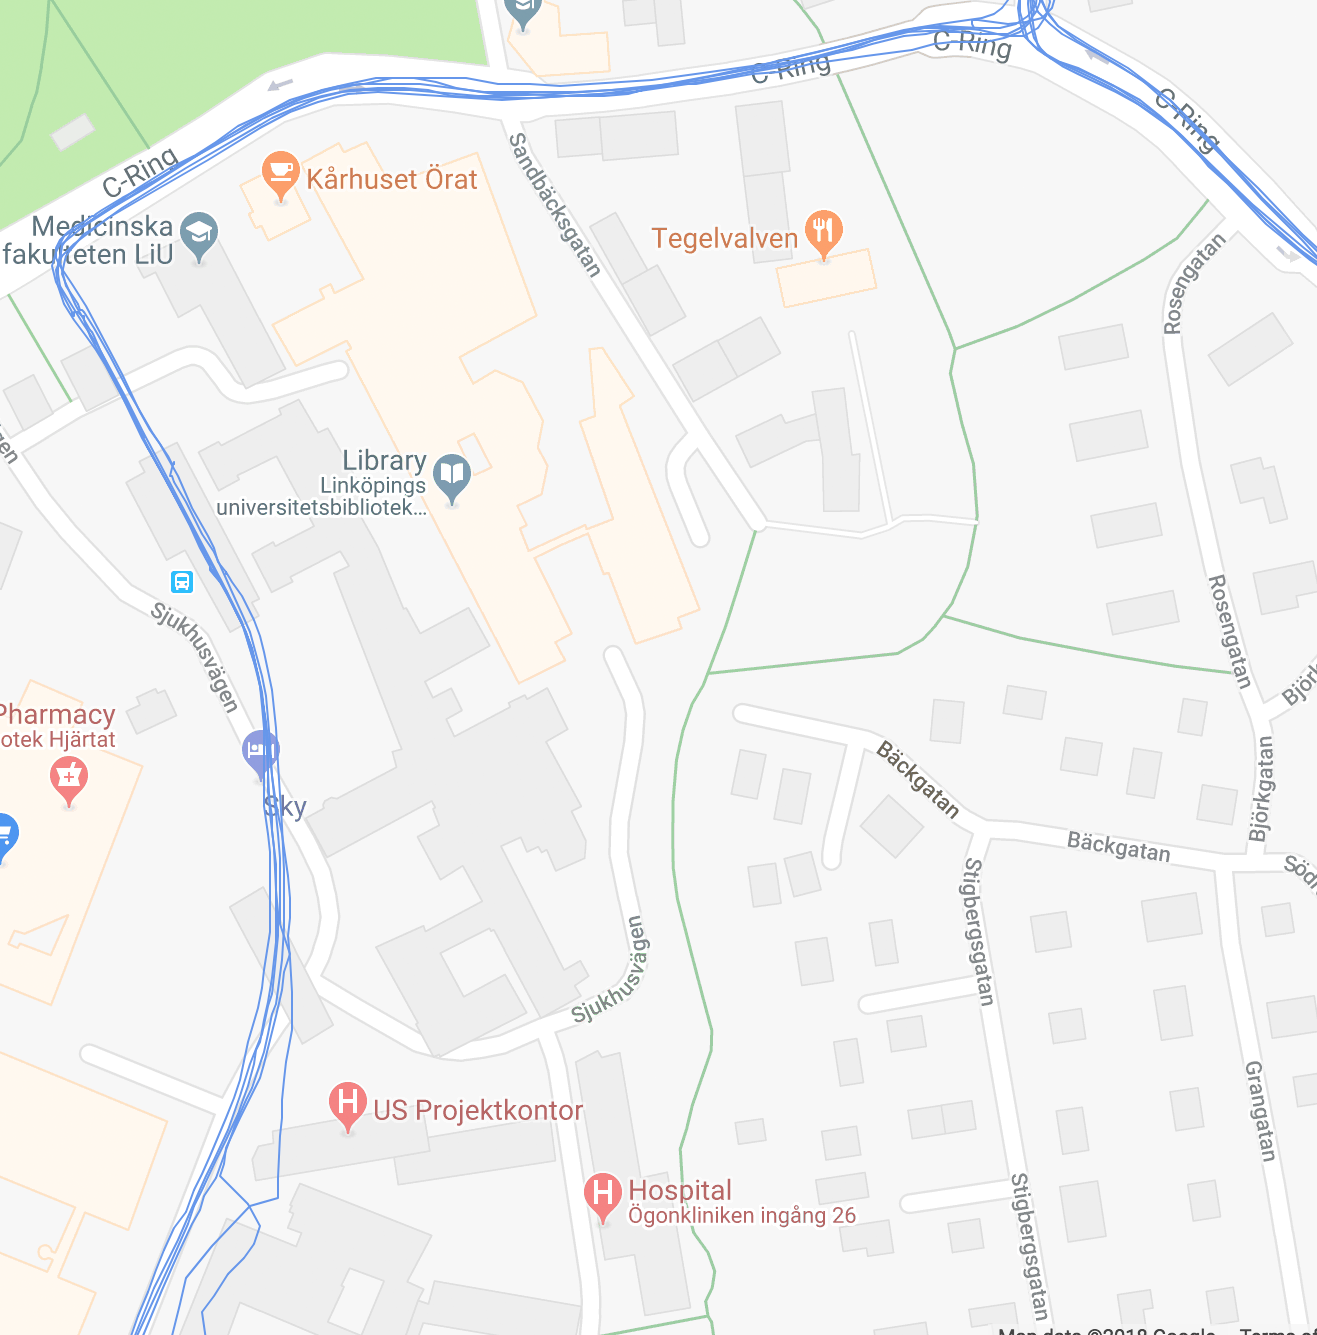
\includegraphics[width=0.9\textwidth]{figures/gps_map_problem}
    \caption[Real-world example of multiple buses driving on a road not correctly modelled by Google Maps]
    {\small Real-world example of multiple buses driving on a road not correctly modelled by Google Maps.
    For example, at "Sjukhusvägen" the buses are driving through a building according to Google Maps.
    In this particular scenario the area has received major road re-structuring and renovation.
    The Google Maps representation is thus likely outdated.}
    \label{fig:gps-map-problem}
\end{figure}

\section{Stop Compression} \label{sec:stop-compression}
Each stop present in the journey causes an imbalance of points being clustered around that stop.
The longer the stop is, the more points are present.
This results in problems when using a GP model, as certain coordinates would thus be denser than others.
The GP would model the noise of the GPS in these denser areas, instead of the variance due to the environment.

Stop compression can be achieved in multiple ways, e.g., stopped positions could be either averaged or ignore completely.
The time of the stop is also adjusted.
In this thesis project, all \texttt{ObservedPositionEvent}s with a \textit{Speed} value lower than $0.1$ m/s were discarded.
The result is a journey (trajectory) consisting of a sequence of coordinates where stops are invisible time-wise.

Examples of the procedure is shown in Figures \ref{fig:uncompressed-events}-\ref{fig:time-and-speed-segment}.
All of the figures show the same trajectory.
Figure \ref{fig:uncompressed-events} shows the trajectory without stop compression, where the stops are highlighted by drawn lines.
Figure \ref{fig:time-and-speed} shows the stop compressed speeds and coordinates of the trajectory.
Figure \ref{fig:time-and-speed-segment} zooms in on an arbitrary segment of the stop compressed trajectory.
The stop compression is implemented using a \textit{Speed} threshold value of $0.1$ m/s.

\begin{figure}[h!]
    \centering
    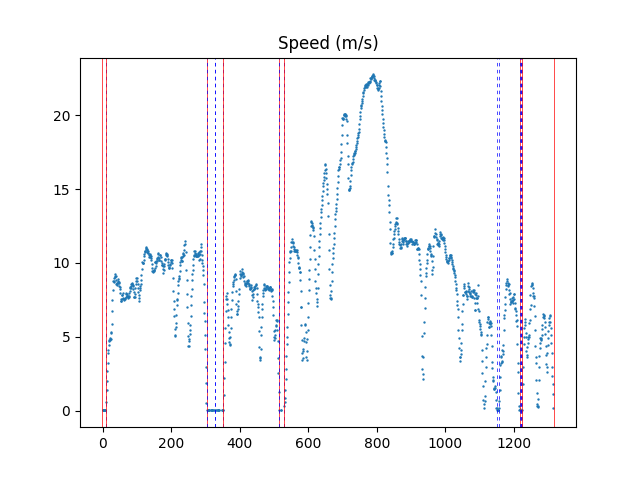
\includegraphics[width=0.9\textwidth]{figures/speed_and_stops_filter_0}
    \caption[Example of a trajectory with uncompressed speeds]
    {\small Example of a trajectory with uncompressed speeds.
    The red lines are \texttt{ArrivedEvent}s and \texttt{DepartedEvent}s.
    The dashed blue lines are \texttt{StartedEvent}s and \texttt{StoppedEvent}s.
    The red and blue lines usually coincide.}
    \label{fig:uncompressed-events}
\end{figure}

\begin{figure}[h!]
    \centering
    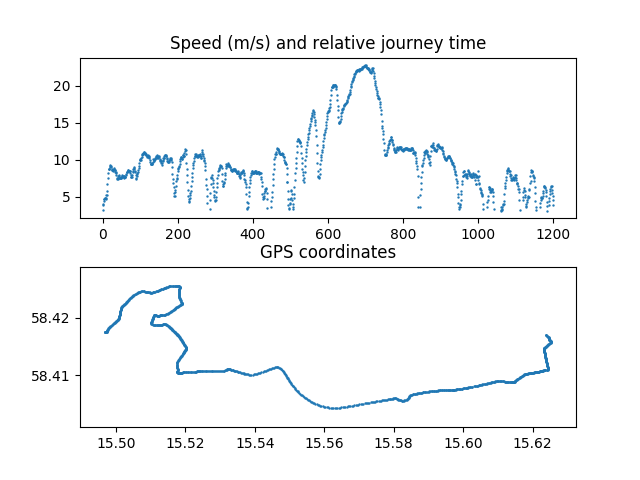
\includegraphics[width=0.9\textwidth]{figures/time_and_speed}
    \caption[Example of a stop compressed trajectory]
    {\small Example of a stop compressed trajectory.
    The \textit{Speed} threshold is set to $0.1$ m/s.
    The various speeds are shown in the top graph, while the trajectory is drawn in the bottom graph.}
    \label{fig:time-and-speed}
\end{figure}

\begin{figure}[h!]
    \centering
    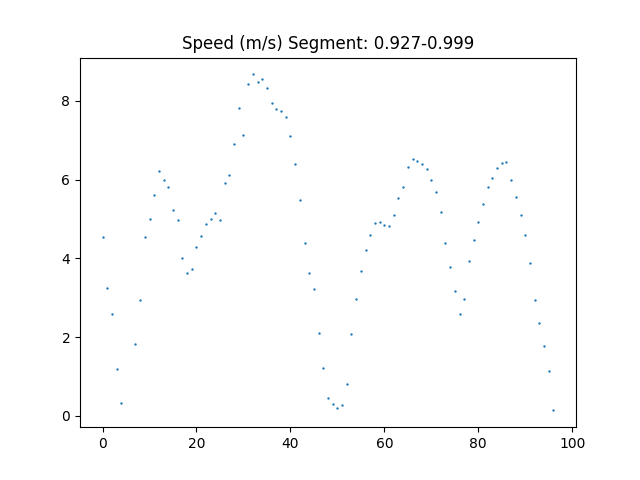
\includegraphics[width=0.8\textwidth]{figures/time_and_speed_segment}
    \caption[Another example of a stop compressed trajectory segment]
    {\small Another example of a stop compressed trajectory segment.
    The duration of a stop causes no delay in the relative time of the trajectory.}
    \label{fig:time-and-speed-segment}
\end{figure}

\section{Synchronising Input Space} \label{sec:synchronisation}
Before GPs can be trained on the journey data, the journeys need to be synchronised in their input space.
A journey can be seen as a sequence of (longitude, latitude, time)-tuples, where \textit{time} is the timestamp of the bus when it is at coordinate (longitude, latitude).
However, at identical values for the \textit{time} parameter, different buses driving for the same bus line have progressed differently on the journey.
For example, buses drive at different speeds and they may stay stopped for different periods of time at each bus stop.
The \textit{time} parameter needs thus to be synchronised, so that (longitude, latitude)-pairs can be compared.
The synchronisation is achieved by introducing a global bus line GP $f_1$, given by

\begin{equation} \label{eq:gps-var-f1}
    f_1: (x, y) \longmapsto \tau,
 \end{equation}
where $(x, y)$ is the (longitude, latitude)-pair and $\tau$ the synchronised \textit{time} parameter.
Each bus line has its own $f_1$ GP, which is trained on a chosen trajectory for that bus line.

Before the model is trained on the trajectory the data is pre-processed with a stricter stop compression algorithm.
Instead of discarding \texttt{ObservedPositionEvent}s with a \textit{Speed} value lower than $0.1$ m/s, the threshold is increased to $3$ m/s.
The reason behind this is to reduce the impact from stops and traffic on the model training.
The trajectory used for the training was arbitrarily chosen from a pool of trajectories occurring in the middle of the night, as during night-time, the buses stop at fewer bus stops and the traffic is lighter.

GP models also assume zero mean for the input data, which in this thesis project is achieved by fitting a global scaler model to the input data.
The same trajectory used for $f_1$ is used to fit this scaler.
All trajectory coordinates are centralised and normalised by the same scaler.
\todo{@Mattias: Homogenously scaled data is good, om jag minns mina praktiska machine learning kurser från ETH}

The GPflow framework \cite{GPflow2017} is used to implement all GP functionality in this thesis work. 

\section{Segment Self-Overlapping Journeys} \label{sec:segment-self-overlapping-journeys}
After the input space synchronisation, each trajectory if fitted with two GPs.
Journeys are analysed in order to detect self-overlapping, which would cause problems for the GP models, as described in Section \ref{sec:self-overlapping-trajectories}.
Journeys with self-overlap are split at the overlapping points into two segments.
The process recursively analyses each resulting segment and proceeds with splitting the segments as long as self-overlapping is present.
If a journey has multiple segments, each segment is fitted with its own two GPs
\begin{align}
    f_2&: \tau \longmapsto x \\
    f_3&: \tau \longmapsto y
\end{align}
$\tau$ is the relative time of the journey, denoting the progress the bus has made on its journey, $x$ the longitude, and $y$ the latitude.
The $\tau$ values are from the $f_1$ GP, evaluated on the trajectory data.

Once $f2_k$ and $f3_k$ have been trained for each trajectory $k$, the GPs are evaluated on a $N$ long interval ($[0,1]$) of $\tau$ values.
The result is a sequence of longitude and latitude means and variances.

\section{Probability Models}
The GPs $f_2$ and $f_3$ each describe the mean ($\mu_x$ and $\mu_y$, respectively) and variance ($\sigma_x^2$ and $\sigma_y^2$, respectively) at each point in the fitted segment or journey.
The probability for various coordinate pairs $p((x_\star,y_\star))$ is of interest in this thesis project, which can be calculated with two different approaches.

\subsection{Mixture of Gaussian Process Model with Uniform Prior}
The first approach is to see all of the trajectory models for the same bus line as a Mixture of Gaussian Process (MoGP) model.
An observed $(x_\star, y_\star)$ coordinate is thus assumed to be generated from one of the GP models in the MoGP.
The prior on the MoGP model is assumed to be Uniform.
The probability of $(x_\star, y_\star)$ for each trajectory model $k$ is 
\(
    p_k((x_\star,y_\star)) = \mathcal{N}((x_\star,y_\star); \mu_k, \Sigma_k)
\)\todo{borde det inte vara $\sim$ istället för $=$?}, where
\begin{align}
\mu_k &= \begin{bmatrix} \mu_{k_x} \\ \mu_{k_y} \end{bmatrix} \\
\Sigma_k &= \begin{bmatrix} \sigma^2_{k_x} & 0 \\ 0 & \sigma^2_{k_y} \end{bmatrix}
\end{align}
is the mean and covariance of the point evaluated at $(x_\star,y_\star)$.
In the covariance matrix $\Sigma_k$, longitude and latitude is assumed to be independent.
As the MoGP prior is Uniform, the probability of $(x_\star, y_\star)$ is given by
\begin{equation}
    p((x_\star, y_\star)) = \frac{1}{K}\sum_{k=1}^K p_k((x_\star,y_\star)) 
\end{equation}

\subsection{Unimodal Mixture of Gaussian Process Model by Combining}
In order to create a unimodal MoGP model, $f_{2_k}$ and $f_{3_k}$ are point-wise combined for each trajectory $k$.
The equations \ref{eq:mean-point-wise-combined} and \ref{eq:var-point-wise-combined} from Section \ref{sec:trajectory-aggregation} are applied as follows:
\begin{align}
    \mu_x(x^*) &= \frac{\sum_{k=1}^{K} M_k\mu_{k_x}(x^*)}{\sum_{k=1}^{K} M_k} \label{eq:combined-mu-x} \\
    \mu_y(y^*) &= \frac{\sum_{k=1}^{K} M_k\mu_{k_y}(y^*)}{\sum_{k=1}^{K} M_k} \label{eq:combined-mu-y} \\
    \sigma_x^2(x^*) &= \frac{\sum_{k=1}^{K} M_k\Big(\sigma_{k_x}^2(x^*) + \mu_{k_x}^2(x^*)\Big)}{\sum_{k=1}^{K} M_k} - \mu_x(x^*)^2 \label{eq:combined-var-x} \\
    \sigma_y^2(y^*) &= \frac{\sum_{k=1}^{K} M_k\Big(\sigma_{k_y}^2(y^*) + \mu_{k_y}^2(y^*)\Big)}{\sum_{k=1}^{K} M_k} - \mu_y(y^*)^2 \label{eq:combined-var-y}
\end{align}
where
\begin{itemize}
    \item $M_k$ is the number of trajectories used to train $f_{2_k}$ and $f_{3_k}$.
    In this thesis project, each trajectory $k$ was trained on its own $f_{2_k}$ and $f_{3_k}$ $\Rightarrow$ $M_k = 1$ for all $k = 1,\dotso,K$ trajectories.
    \item $x^*$ and $y^*$ are index slices (points) to evaluate the MoGP model at.
    \item $\mu_{k_x}$ and $\mu_{k_y}$ is the predicted mean of the evaluated point at the index slice of x (longitude) and y (latitude), respectively. 
    \item $\sigma_{k_x}^2$ and $\sigma_{k_y}^2$ is the predicted variance of the evaluated point at the index slice. 
\end{itemize}

Equations \ref{eq:combined-mu-x}-\ref{eq:combined-var-y} can thus be simplified to
\begin{align}
    \mu_x(x^*) &= \frac{\sum_{k=1}^{K} \mu_{k_x}(x^*)}{K} \label{eq:simplified-combined-mu-x} \\
    \mu_y(y^*) &= \frac{\sum_{k=1}^{K} \mu_{k_y}(y^*)}{K} \label{eq:simplified-combined-mu-y} \\
    \sigma_x^2(x^*) &= \frac{\sum_{k=1}^{K} \Big(\sigma_{k_x}^2(x^*) + \mu_{k_x}^2(x^*)\Big)}{K} - \mu_x(x^*)^2 \label{eq:simplified-combined-var-x} \\
    \sigma_y^2(y^*) &= \frac{\sum_{k=1}^{K} \Big(\sigma_{k_y}^2(y^*) + \mu_{k_y}^2(y^*)\Big)}{K} - \mu_y(y^*)^2 \label{eq:simplified-combined-var-y}
\end{align}

The equations \ref{eq:simplified-combined-mu-x}-\ref{eq:simplified-combined-var-y} give the combined unimodal MoGP model at index slice $(x^*, y^*)$
\begin{align}
\mu((x^*, y^*)) &= \begin{bmatrix} \mu_x(x^*) \\ \mu_y(y^*) \end{bmatrix} \\
\Sigma((x^*, y^*)) &= \begin{bmatrix} \sigma^2_x(x^*) & 0 \\ 0 & \sigma^2_y(y^*) \end{bmatrix}
\end{align}
which gives the probability of an arbitrary point $(x_\star, y_\star)$: $p(x_\star, y_\star) = \mathcal{N}((x_\star, y_\star), \mu, \Sigma)$
\todo{@Mattias: Är osäker på exakt hur jag ska formulera matematiskt det vi gör. Försöker hitta liknande notaitoner i litteraturen, men finner inget bra exempel.}

\section{Results}

The unimodal MoGP model is visualised by evaluating the MoGP model on a grid of (longitude, latitude) values.
Figure \ref{fig:predictive-mean-combined-gp} shows the predictive mean for the unimodal MoGP model.
The trajectory shown is thus the predicted mean of observing new data points for the bus line.
The MoGP model consists of 37 trajectories from a single day. 
Figure \ref{fig:predictive-var-combined-gp1} shows the predictive variance of the starting segment for the bus line and Figure \ref{fig:starting-segment-trajectory} shows this starting segment on Google Maps, where the red lines are trajectories for the bus line.
Figure \ref{fig:fig:predictive-var-combined-gp2} shows a predictive variance for a segment of the trajectory containing a bus stop.
\begin{figure}[t!]
    \centering
    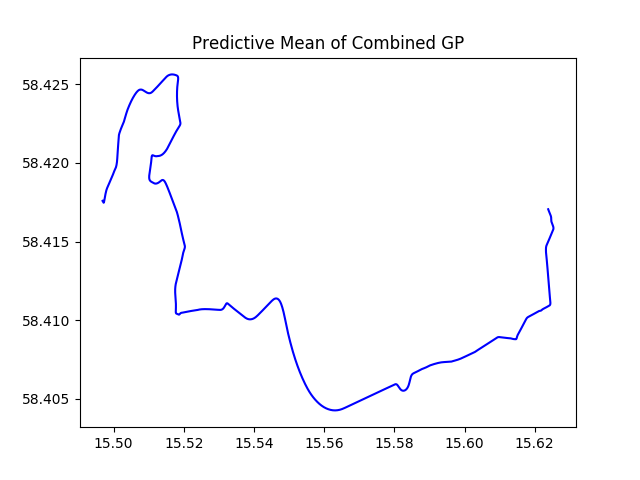
\includegraphics[width=0.9\textwidth]{figures/combined_gp}
    \caption[Predictive mean of the unimodal MoGP model]
    {\small Predictive mean of the unimodal MoGP model. 
    The trajectory shown is the mean trajectory of 37 trajectories.}
    \label{fig:predictive-mean-combined-gp}
\end{figure}

\begin{figure}[h!]
    \centering
    \begin{subfigure}[t]{0.6\textwidth}
        \centering
        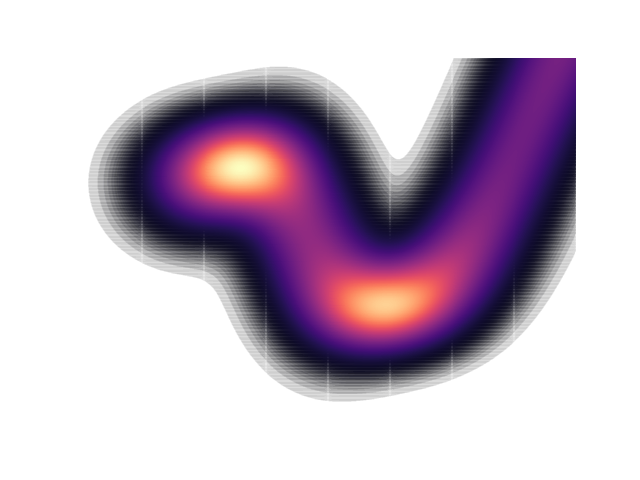
\includegraphics[width=\textwidth]{figures/0_1000x1000}
        \caption[Heatmap of the predictive variance of the unimodal MoGP model]
        {\small Heatmap of the predictive variance of the unimodal MoGP model.}
        \label{fig:predictive-var-combined-gp1}
    \end{subfigure}
    ~
    \begin{subfigure}[t]{0.5\textwidth}
        \centering
        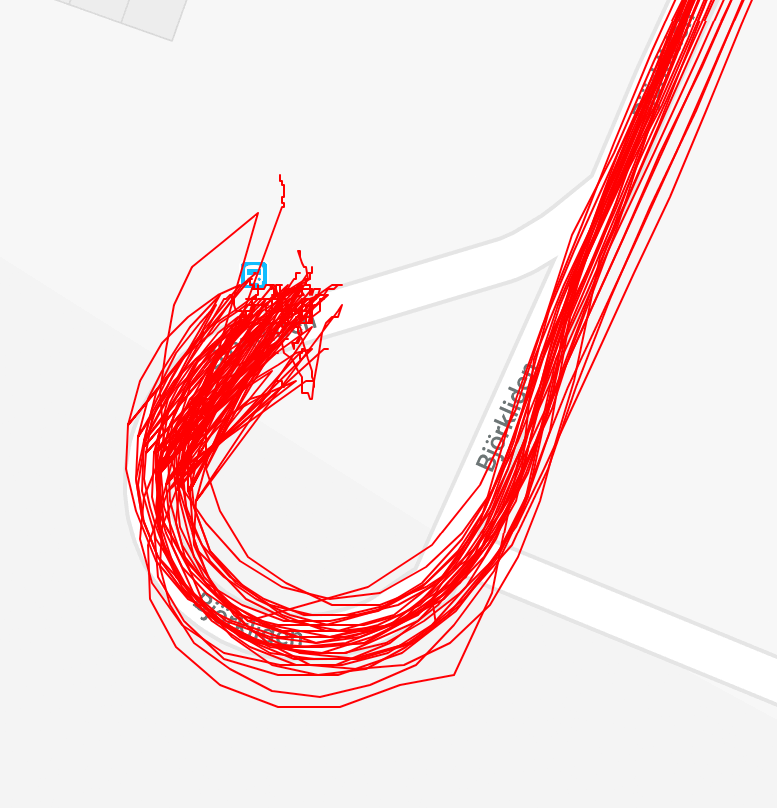
\includegraphics[width=\textwidth]{figures/starting_segment}
        \caption[]
        {\small Starting segment with bus line journeys (trajectories) drawn with red lines.}
        \label{fig:starting-segment-trajectory}
    \end{subfigure}
    \caption[The predictive variance and the trajectories for the starting segment $S_0$]
    {\small The predictive variance and the trajectories for the starting segment $S_0$.}
\end{figure}

\begin{figure}[h!]
    \centering
    \begin{subfigure}[t]{0.9\textwidth}
        \centering
        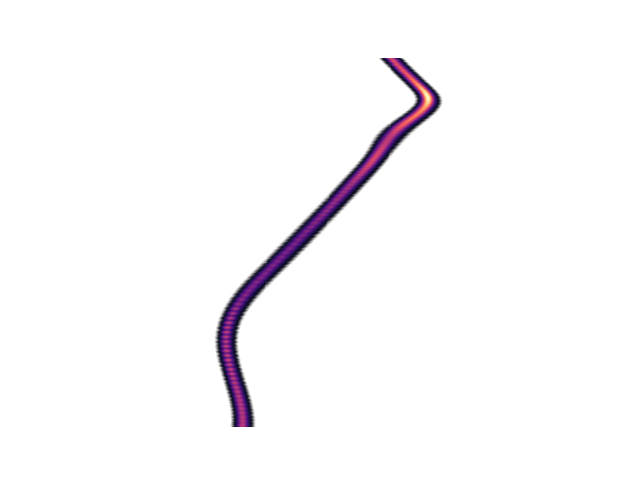
\includegraphics[width=\textwidth]{figures/2_1000x1000}
        \caption[]
        {\small Segment containing a bus stop.
        The bus stop occurs immediately after top curve.}
    \end{subfigure}
    ~
    \begin{subfigure}[t]{0.9\textwidth}
        \centering
        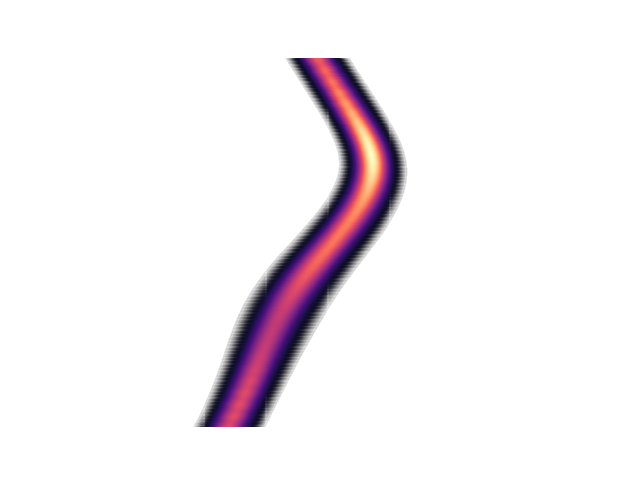
\includegraphics[width=\textwidth]{figures/3_1000x1000}
        \caption[]
        {\small The bus stop is zoomed in to show the increase in predictive variance around the bus stop.}
    \end{subfigure}
    \caption[Predictive variance of the unimodal MoGP model]
    {\small Predictive variance of the unimodal MoGP model.
    The segment shown contains a bus stop.}
    \label{fig:predictive-var-combined-gp2}
\end{figure}

\section{Discussion}

\section{Future Work}